\documentclass[11pt,letterpaper]{article}
%\documentclass[11pt,a4paper]{report}


\usepackage{tikz}
\usepackage{amssymb,amsmath,amsthm} 
\usepackage[margin=2cm]{geometry}
\usepackage{fancyhdr}
\usepackage{enumitem}
\usepackage[compact]{titlesec}
\usepackage{graphicx,ctable,booktabs,subcaption}

\usepackage{xparse,hyperref,parskip}

%\newcommand{\abs}[1]{\left|#1\right|}

\newcommand{\semester}{Spring 2022}
\newcommand{\due}{Thursday, March 24}

\newcommand{\bigo}{\mathcal{O}}

\pagestyle{fancy}
\lhead{ }
\chead{\footnotesize Math 3338\quad  Numerical Methods\quad  \semester}
\rhead{\footnotesize \thepage}
\setlength{\parindent}{0cm}
\setlist{noitemsep}



\newtheorem{theorem}{Theorem}

\input{defs.tex}

%Defines the problem environment with arguments Points and Solution gap
\input{problem_env.tex}



\begin{document}

\begin{center}
{\huge{\bf  Numerical Methods}} \\[1.5ex]
{\bf Math 3338 -- \semester}\\[1.5ex]
{\Large{\bf Worksheet 18 \\[2ex] Networkx}}\\
\end{center}
\vspace{2mm}


\section{Reading}

\begin{table}[!ht]
 \centering
 \begin{tabular}{ll}
   CP &  8.1, 8.2 \\
 NMEP &  Chapter 7
 \end{tabular}
\caption{Sections Covered}
\end{table}






\section{Graphs}
A graph $G=(V,E)$ consists of two sets, $V$ is the set of vertices and $E\subseteq\binom{V}{2}$ is
the set of edges. The notation $\binom{V}{2}$ may be new to you, it just choosing two element from
$V$, so it's all subsets of size $2$. We'll be dealing with simple graphs, graphs with are
undirected, with no multiple edges and no loops. We'll see that the adjacency matrix of simple
graphs are symmetric with 0's on the diagonal. Figure \ref{fig:exa_graph} has an example of a graph.

\begin{figure}[!ht]
 \centering
 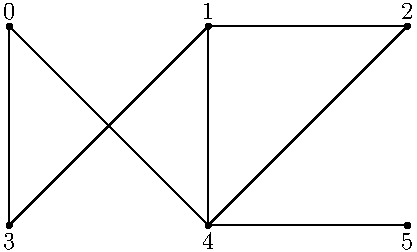
\includegraphics{images/exa_graph.pdf}
 \caption{A graph!}
 \label{fig:exa_graph}  
\end{figure}


Let's call the graph in Figure \ref{fig:exa_graph} $G_1$. There are several ways we can represent this
graph in Python. First, we can use a dictionary,
\begin{verbatim}
G1 = { 0:[3,4],
       1:[2,3,4],
       2:[1,4],
       3:[0,1],
       4:[0,1,2,5],
       5:[4]
     }
\end{verbatim}
The keys are the vertices and the values are a list of the neighbors of the vertex. A neighbor is a
vertex that is adjacent (connected) to the given vertex. This representation has several advantages. 
The most notable is that the vertices don't need to be integers they could be strings, tuples
or any non-mutable type. It's also easy to compute the degree sequence,
\begin{verbatim}
[len(value) for value in G1.values()]
\end{verbatim}
This is the sequence of degrees of each vertex, or the number of neighbors of each vertex.


Another way to represent this graph is as a matrix. 
\begin{equation*}
 A = \begin{bmatrix}
0 & 0 & 0 & 1 & 1 & 0  \\
0 & 0 & 1 & 1 & 1 & 0  \\
0 & 1 & 0 & 0 & 1 & 0  \\
1 & 1 & 0 & 0 & 0 & 0  \\
1 & 1 & 1 & 0 & 0 & 1  \\
0 & 0 & 0 & 0 & 1 & 0 
\end{bmatrix}
\end{equation*}
The adjacency matrix is a matrix consisting of $0$'s and $1$'s, where $a_{ij}=1$ if the vertices
$i$ and $j$ are adjacent. As may be apparent this is far more difficult to manually input. Also, the
vertices are implicitly ordered, which is important to keep in mind. It's actually still very simple
to get the degree sequence of this graph.
\[
A\cdot\vec{1}
\]
Where $\vec{1}$ is a column vector of $1$'s. You should very carefully think about why this works.

The adjacency matrix is much easier to do math on, as it's a matrix. However, the dictionary is much
easier to input an check correctness. The solution is to write a function that converts a dictionary
to an adjacency matrix. 

\begin{verbatim}
def adjacency_matrix(graph):
    vertices = sorted(graph) #Set an order on the vertices
    N = len(vertices)
    A = np.zeros((N,N))
    for i,vert in enumerate(vertices):
        for j in [vertices.index(elm) for elm in graph[vert]]:
            A[i,j] += 1
    return A    
\end{verbatim}

This code should be able to handle any graph whose vertices can be sorted (I only tested on 
integers). 

\section{The Adjacency Matrix}
Let $A=(a_{ij})$ be the adjacency matrix. The $a_{ij}$ is the number of paths from $v_i$ to $v_j$
of length 1. It's telling you if they are connected. If $A^2=(b_{ij})$ then $b_{ij}$ is the number
of paths from $v_i$ to $v_j$ of length 2. Using the graph in Figure \ref{fig:exa_graph} we see
$b_{01}=2$, there are two paths from $0$ to $1$. This generalizes, the entries of $A^n$ are the
number of paths of length $n$.



\section{NetworkX}
NetworkX provides data structures for graphs along with graph algorithms, generators, and drawing tools. Load the NetworkX package using \texttt{import networkx as nx}. The best resource for NetworkX is their documentation \url{https://networkx.org/documentation/networkx-1.10/reference/introduction.html}. 


Here is some sample code to generate a barbell graph (two complete graphs connected by a path), the average clustering of this graph, and finally draw it.
\begin{verbatim}
import networkx as nx

G = nx.barbell_graph(5,4)

print(nx.average_clustering(G))
nx.draw(G)
\end{verbatim}
Notice the drawing is... not great. We'll discuss this in more detail next time. 

You can also define a graph from a dictionary
\begin{verbatim}
H = nx.Graph({0:[1,2],1:[1,2],2:[0,1]})
\end{verbatim}
and many other methods. 


\section{Graph Statistics}
Not like mean and standard deviation, but numbers that describe graphs. You've seen one, average clustering, but what is average clustering and what are more?

\texttt{average\_clustering} - This is the average of the local clustering coefficients. For a vertex $v\in V$ the neighborhood of $v$ is the set $N_v = \{u\in V\st (u,v) \in E\}$, in other words it's all the vertices connected to $v$. The the local clustering coefficient of $v$ is 
\[
 C_v = \frac{2\abs{\{(u,w)\in E\, |\, u,w\in N_v\}}}{\abs{N_v}\abs{N_v-1}}.
\]
Essentially, the local clustering coefficient is the ratio of the number of connections between the neighbors of $v$ and the total number of possible connections.\footnote{The 2 in the numerator disappears for directed graphs. Do you know why?} The average clustering is then,
\[
C = \frac{1}{\abs{V}}\sum_{v\in V} C_v
\]
For example, for the graph in Figure \ref{fig:exa_graph} the clustering coefficient of $1$ is $\frac{1}{3}$. You can find the local clustering of each vertex using \texttt{nx.clustering(G)}. Why is this useful? Think social networks. How many of your friends are friends? Could this be used to determine if your friends should be friends?


\texttt{betweeness\_centrality} - For a vertex $v\in V$, what is the ratio ``shortest paths'' between pairs of vertices that pass through $v$ vs all shortest paths? In math terms, if $\sigma_{s,t}$ is the number of shortest paths from $s$ to $t$ and $\sigma_{s,t}(v)$ is the number that pass through $v$ then,
\[
C_{between}(v) = \sum_{s,t\in V} \frac{\sigma_{s,t}(v)}{\sigma_{s,t}}.
\]
For example, in Figure \ref{fig:exa_graph} $C_{between}(1) = \frac{1}{5}$. You should try to verify this by hand\footnote{It's really, really hard}. This is an informative statistic, but it's $\mathcal{O}(n^3)$, or quite slow. 


\texttt{eccentricity} - For a vertex $v\in V$ the eccentricity of $v$ is the maximum shortest distance between $v$ and any other vertex $u\in V$. For example, the eccentricity of $1$ in Figure \ref{fig:exa_graph} is 2. The \texttt{diameter} of a graph is the maximum eccentricity and the \texttt{radius} is the minimum eccentricity. 





\newpage

\begin{center}
{\huge{\bf  Numerical Methods}} \\[1.5ex]
{\bf Math 3338 -- \semester}\\[1.5ex]
{\Large{\bf Homework 18 (Due: \due)}}\\
\end{center}
\vspace{2mm}

For these problems you'll be submitting a PDF on Canvas. 

\begin{problem}
 Without using Python, what are the following for the complete graph $K_5$?
 \begin{itemize}
  \item average clustering
  \item betweeness centrality (for any vertex)
  \item eccentricity (for any vertex)
  \item diameter
  \item radius
 \end{itemize}
 Justify your answers and check using Python. 
\end{problem}


For the Problems \ref{prob:start}--\ref{prob:end} refer to Figure \ref{fig:prob}.
\begin{figure}[!ht]
 \centering
 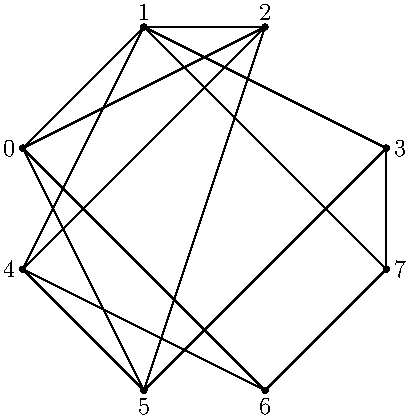
\includegraphics{images/problem_02.pdf}
 \caption{For some problems}
 \label{fig:prob}  
\end{figure}


\begin{problem}
 \label{prob:start}
 Find the following. Also draw the graph with the vertices labeled. 
  \begin{itemize}
   \item average clustering
   \item betweeness centrality (for any vertex)
   \item eccentricity (for any vertex)
 \item diameter
 \item radius
  \end{itemize}
\end{problem} 


\begin{problem}
 \label{prob:end}
 What, in your opinion, is the most important and least important vertex in this graph? Justify your answer.
\end{problem} 


\begin{problem}
 NetworkX can also generate random graphs. Let's use the \texttt{gnm\_random\_graph(n,m)} function, $n$ is the number of vertices and $m$ the number of edges. Let $n= 50$, iterate $m$ over the list \texttt{[50,100,150,200,250, $\dots$, 800]} and compute the average clustering, diameter, and radius. Make a table with the number of edges and the three statistics. What do you observe about each as the number of edges increases?
\end{problem}



\end{document}





































